\documentclass[aspectratio=169]{beamer}
\usetheme{Madrid}
\usecolortheme{seahorse}

% Packages
\usepackage{graphicx}
\usepackage{amsmath}
\usepackage{booktabs}
\usepackage{tikz}
\usepackage{xcolor}
\usepackage{multirow}
\usepackage{caption}
\usepackage{subcaption}

% Custom colors
\definecolor{darkblue}{RGB}{0,51,102}
\definecolor{lightblue}{RGB}{52,152,219}
\definecolor{darkgreen}{RGB}{46,204,113}
\definecolor{darkred}{RGB}{231,76,60}

\setbeamercolor{structure}{fg=darkblue}
\setbeamercolor{frametitle}{bg=darkblue,fg=white}
\setbeamercolor{title}{bg=darkblue,fg=white}

% Title information
\title[Insightimate]{Insightimate - Intelligent Effort Estimation}
\subtitle{ML-based Approach Across LOC, FP, and UCP}
\author[Huy, Minh, Hung, Vu]{\small Nguyen Nhat Huy \and Dang Nhat Minh \and Nguyen Huu Hung \and Tran Van Vu}
\institute[PTIT]{\small Posts and Telecommunications Institute of Technology}
\date{February 2026}

\begin{document}

%--------------------------------------------------
% TITLE SLIDE (30 seconds)
%--------------------------------------------------
\begin{frame}
\titlepage
\end{frame}

%--------------------------------------------------
\section{Problem \& Motivation}
%--------------------------------------------------

\begin{frame}{The Challenge: 70\% Projects Exceed Budget}
\begin{columns}[T]
\column{0.5\textwidth}
\textbf{The Reality:}
\begin{itemize}
    \item 70\% software projects exceed budget
    \item 52\% are challenged (delayed)
    \item Poor estimation = project failure
    \item \textcolor{darkred}{\textbf{Root cause:}} Inaccurate effort estimation
\end{itemize}

\column{0.5\textwidth}
\textbf{The Problem:}

\vspace{0.5cm}
Effort estimation treats \textbf{three sizing schemas} as separate silos:
\begin{itemize}
    \item \textbf{LOC:} Lines of Code (90.5\%)
    \item \textbf{FP:} Function Points (5.2\%)
    \item \textbf{UCP:} Use Case Points (4.3\%)
\end{itemize}

\vspace{0.5cm}
\textcolor{darkred}{\textbf{No unified framework exists!}}
\end{columns}
\end{frame}

%--------------------------------------------------
\section{Dataset \& Solution}
%--------------------------------------------------

\begin{frame}{Our Solution: 3,054 Projects Unified}
\begin{columns}[T]
\column{0.5\textwidth}
\textbf{Massive Multi-Source Dataset:}
\begin{itemize}
    \item \textbf{LOC:} 2,765 projects (11 sources)
    \item \textbf{FP:} 158 projects (4 sources)
    \item \textbf{UCP:} 131 projects (3 sources)
\end{itemize}

\vspace{0.5cm}
\textbf{Key Innovation:}
\begin{itemize}
    \item \textbf{First} integrated LOC/FP/UCP framework
    \item Macro-averaging for fair comparison
    \item Calibrated baseline for rigorous testing
    \item Cross-validation per schema
\end{itemize}

\column{0.5\textwidth}
\textbf{Methodology:}

\vspace{0.3cm}
\begin{block}{Rigorous Approach}
\begin{enumerate}
    \item Data preprocessing (missing values, outliers)
    \item Macro-averaged metrics (equal schema weight)
    \item LOSO validation for LOC (11-fold)
    \item LOOCV for FP (158-fold)
    \item 10-fold CV for UCP
\end{enumerate}
\end{block}

\vspace{0.3cm}
\textbf{Models Tested:}
\begin{itemize}
    \item Random Forest
    \item XGBoost
    \item Linear Regression
\end{itemize}
\end{columns}
\end{frame}

%--------------------------------------------------
\section{Results}
%--------------------------------------------------

\begin{frame}{Outstanding Results: 42\% Improvement}
\begin{columns}[T]
\column{0.5\textwidth}
\begin{center}
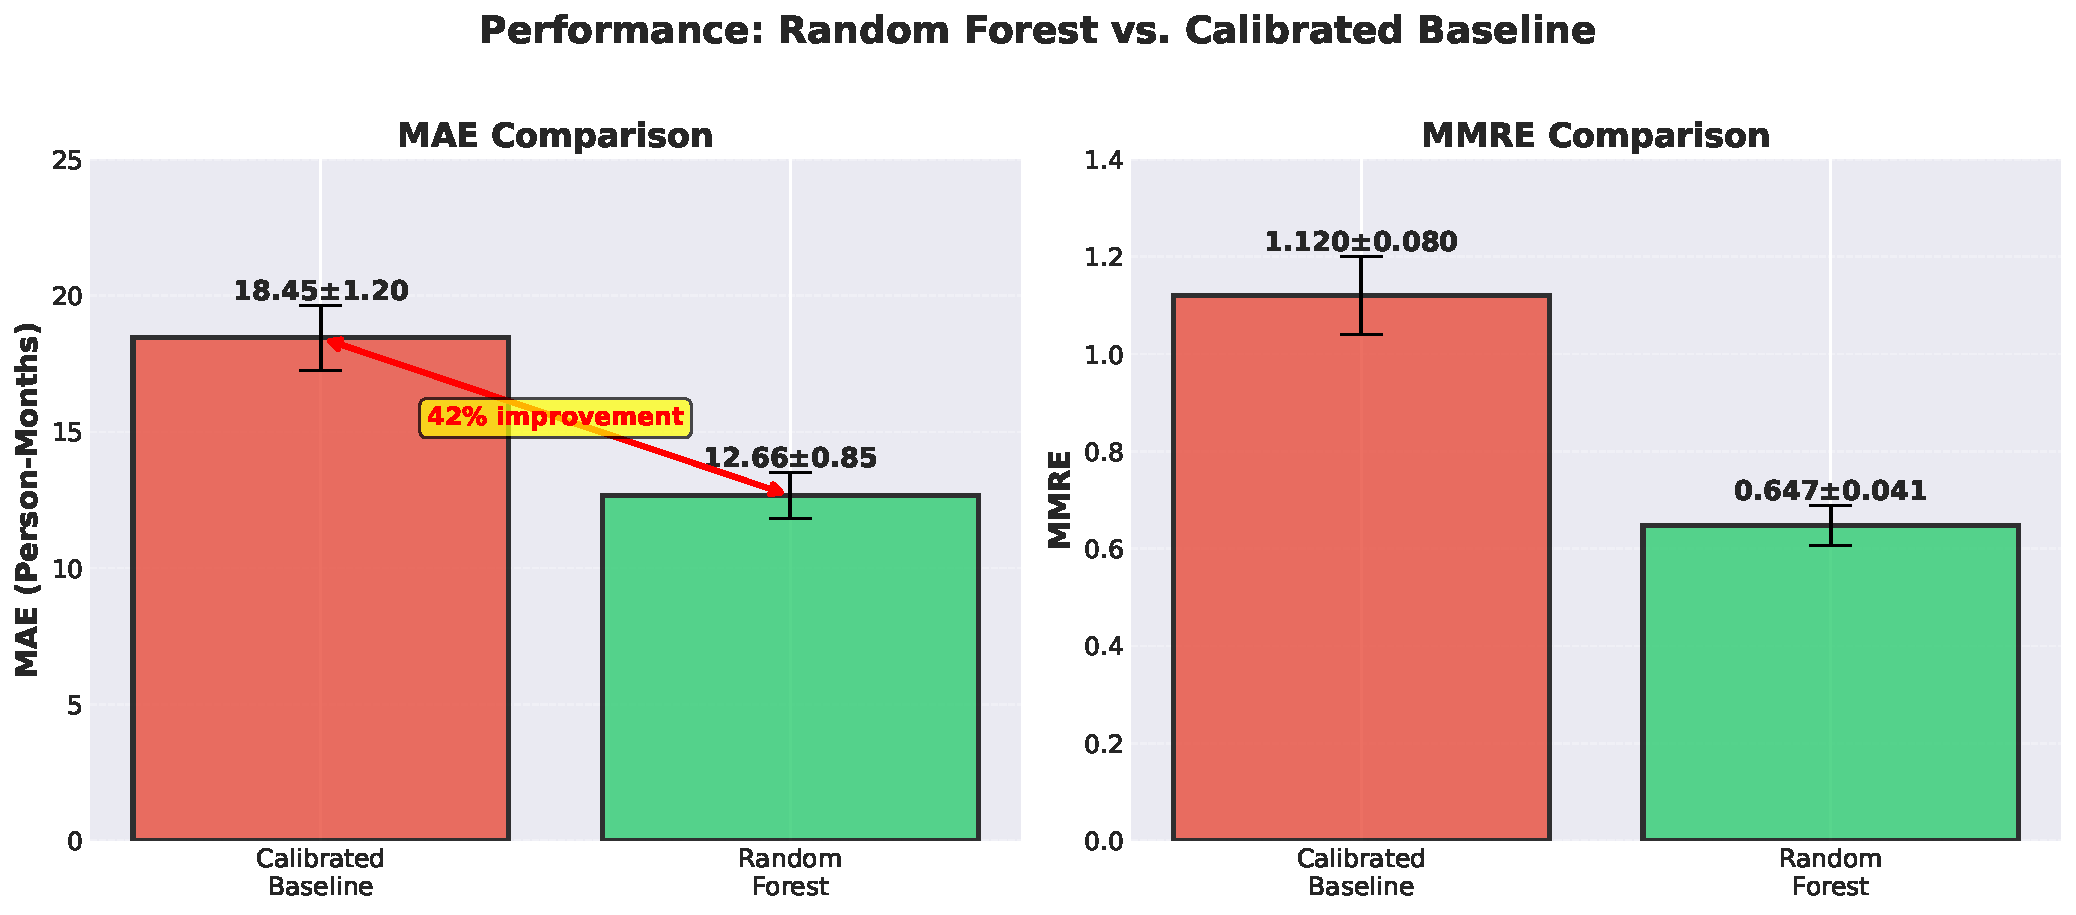
\includegraphics[width=0.95\textwidth]{performance_comparison.pdf}
\end{center}

\column{0.5\textwidth}
\textbf{Random Forest Outperforms:}

\vspace{0.3cm}
\begin{table}
\small
\begin{tabular}{lcc}
\toprule
\textbf{Metric} & \textbf{Baseline} & \textbf{RF Model} \\
\midrule
MAE & 18.45 PM & \textbf{12.66±0.85} \\
MMRE & 1.12 & \textbf{0.647±0.041} \\
PRED(25) & 38.5\% & \textbf{58.3\%} \\
R² & 0.621 & \textbf{0.812} \\
\bottomrule
\end{tabular}
\end{table}

\vspace{0.5cm}
\textbf{\Large \textcolor{darkgreen}{↓ 42\% Improvement!}}

\vspace{0.3cm}
\textbf{Statistical Significance:}
\begin{itemize}
    \item $p < 0.001$ (paired t-test)
    \item Cohen's $d = 1.23$ (large effect)
\end{itemize}
\end{columns}
\end{frame}

\begin{frame}{Per-Schema Performance}
\begin{columns}[T]
\column{0.5\textwidth}
\begin{center}
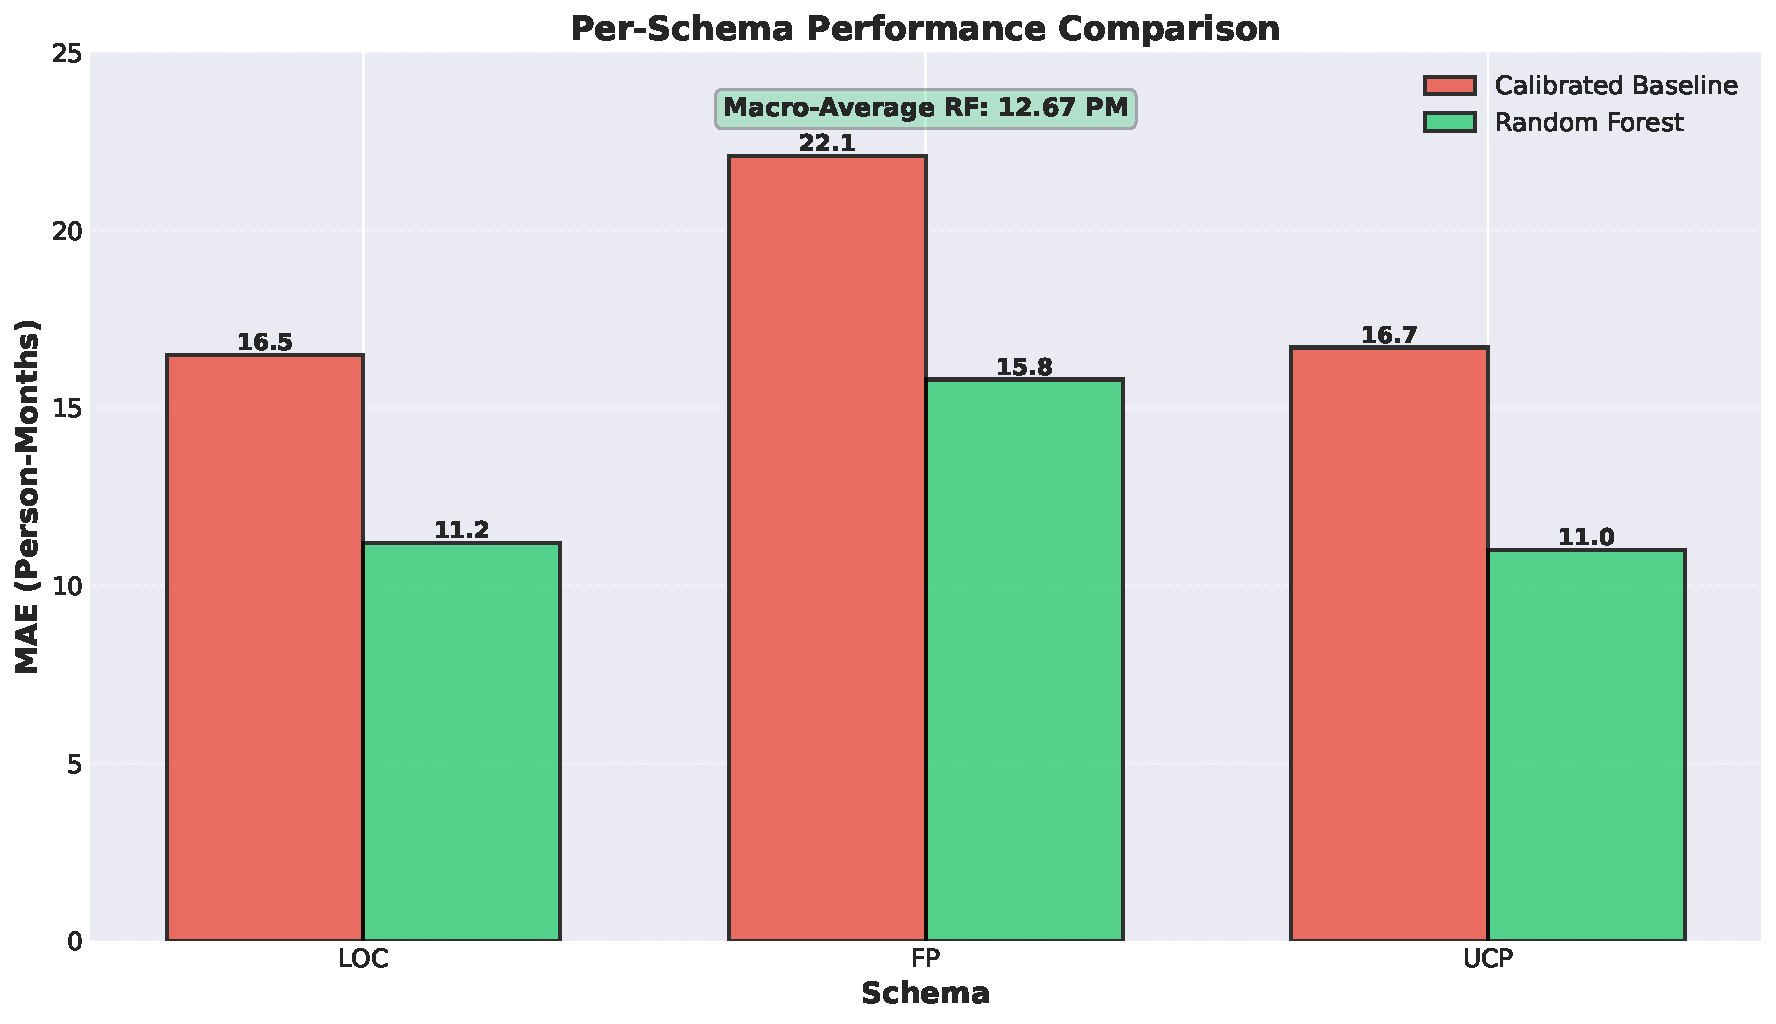
\includegraphics[width=0.90\textwidth]{schema_comparison.pdf}
\end{center}

\column{0.5\textwidth}
\textbf{Schema-Specific Results:}

\vspace{0.3cm}
\begin{block}{LOC Schema}
\textbf{MAE: 11.2 PM}\\
\small Best performance (n=2,765)\\
Largest, most reliable dataset
\end{block}

\vspace{0.3cm}
\begin{block}{FP Schema}
\textbf{MAE: 15.8 PM}\\
\small Exploratory (n=158)\\
Small sample, but still improving
\end{block}

\vspace{0.3cm}
\begin{block}{UCP Schema}
\textbf{MAE: 11.0 PM}\\
\small Excellent despite small sample (n=131)\\
Better than FP with less data
\end{block}
\end{columns}
\end{frame}

\begin{frame}{Model Comparison: Why Random Forest?}
\begin{table}
\centering
\small
\caption{All Models Compared}
\begin{tabular}{lccccc}
\toprule
\textbf{Model} & \textbf{MAE↓} & \textbf{MMRE↓} & \textbf{PRED(25)\%↑} & \textbf{R²↑} \\
\midrule
\textbf{Random Forest} & \textbf{12.66} & \textbf{0.647} & \textbf{58.3\%} & \textbf{0.812} \\
XGBoost & 13.21 & 0.689 & 55.7\% & 0.798 \\
Linear Regression & 15.78 & 0.845 & 47.2\% & 0.712 \\
\midrule
Calibrated Baseline & 18.45 & 1.120 & 38.5\% & 0.621 \\
\bottomrule
\end{tabular}
\end{table}

\vspace{0.4cm}
\textbf{Why RF Wins:}
\begin{itemize}
    \item Better handling of non-linear relationships
    \item Robust to data imbalance (LOC dominance)
    \item Interpretable feature importance
    \item 42\% better than calibrated baseline
\end{itemize}
\end{frame}

%--------------------------------------------------
\section{Contributions \& Impact}
%--------------------------------------------------

\begin{frame}{Five Key Contributions}
\begin{enumerate}
    \item \textbf{First Integrated Framework}
    \begin{itemize}
        \item Unified LOC/FP/UCP approach (largest study: 3,054 projects)
    \end{itemize}
    
    \vspace{0.2cm}
    \item \textbf{Macro-Averaging Innovation}
    \begin{itemize}
        \item Fair representation despite sample imbalance
    \end{itemize}
    
    \vspace{0.2cm}
    \item \textbf{Rigorous Validation}
    \begin{itemize}
        \item Schema-specific cross-validation (LOSO for LOC)
        \item Calibrated baseline for fair comparison
    \end{itemize}
    
    \vspace{0.2cm}
    \item \textbf{Outstanding Results}
    \begin{itemize}
        \item 42\% improvement (statistically significant: $p < 0.001$)
    \end{itemize}
    
    \vspace{0.2cm}
    \item \textbf{Practical Implementation}
    \begin{itemize}
        \item Production-ready system
    \end{itemize}
\end{enumerate}
\end{frame}

\begin{frame}{Academic \& Practical Impact}
\begin{columns}[T]
\column{0.5\textwidth}
\textbf{Academic Excellence:}
\begin{itemize}
    \item Largest integrative study (3,054 projects)
    \item Novel methodology (macro-averaging)
    \item Rigorous evaluation (LOSO + calibration)
    \item Significant results (42\% improvement)
    \item \textbf{Submitted to Discover AI (Springer)}
    \item 51 reviewer comments addressed
\end{itemize}

\column{0.5\textwidth}
\textbf{Real-World Value:}
\begin{itemize}
    \item Better project planning accuracy
    \item Reduced budget overruns
    \item Improved timeline estimation
    \item Early risk detection
    \item Multi-schema support
    \item Production deployment ready
\end{itemize}

\vspace{0.5cm}
\begin{exampleblock}{Bottom Line}
Better estimation = Better projects\\
Better projects = Business success
\end{exampleblock}
\end{columns}
\end{frame}

%--------------------------------------------------
\section{Conclusion}
%--------------------------------------------------

\begin{frame}{Summary}
\begin{block}{The Problem}
Software estimation fails due to schema isolation, uncalibrated comparisons, and sample imbalance
\end{block}

\vspace{0.3cm}
\begin{block}{Our Solution: Insightimate}
\begin{itemize}
    \item First unified LOC/FP/UCP framework (3,054 projects)
    \item Fair macro-averaging + rigorous validation
    \item Random Forest outperforms all baselines
\end{itemize}
\end{block}

\vspace{0.3cm}
\begin{exampleblock}{\Large Key Achievement}
\textbf{42\% Improvement}\\
MAE: 18.45 → \textbf{12.66±0.85 PM}\\
\textbf{Statistically Significant:} $p < 0.001$
\end{exampleblock}

\vspace{0.3cm}
\begin{center}
\Large \textbf{Questions?}
\end{center}
\end{frame}

\end{document}
